%!TEX program = pdflatex
\documentclass[11pt, a4paper]{article}

%% ──────────────────────────────────────────────
%%  Packages
%% ──────────────────────────────────────────────
\usepackage[T1]{fontenc}
\usepackage[utf8]{inputenc}
\usepackage{geometry}
\geometry{a4paper, top=2.5cm, bottom=2.5cm, left=2.5cm, right=2.5cm}

\usepackage{amsmath, amssymb}
\usepackage{graphicx}
\usepackage{xcolor}
\usepackage{hyperref}
\usepackage{booktabs}
\usepackage{array}
\usepackage{enumitem}
\usepackage{parskip}
\usepackage{float}
\usepackage{caption}
\usepackage{titlesec}
\usepackage{fancyhdr}
\usepackage{tcolorbox}
\usepackage{listings}
\usepackage{tikz}
\usepackage{mdframed}
\usepackage{setspace}

\usetikzlibrary{angles, quotes, arrows.meta, calc, shapes.geometric, positioning}
\tcbuselibrary{skins, breakable, listings}

%% ──────────────────────────────────────────────
%%  Colors
%% ──────────────────────────────────────────────
\definecolor{pyblue}{RGB}{0, 80, 160}
\definecolor{pygreen}{RGB}{0, 128, 0}
\definecolor{pyred}{RGB}{180, 30, 30}
\definecolor{pygray}{RGB}{100, 100, 100}
\definecolor{pystring}{RGB}{150, 20, 20}
\definecolor{pycomment}{RGB}{60, 120, 130}
\definecolor{pykeyword}{RGB}{0, 100, 0}
\definecolor{codebg}{RGB}{248, 248, 252}
\definecolor{codeborder}{RGB}{200, 200, 220}
\definecolor{tipbg}{RGB}{240, 248, 255}
\definecolor{tipborder}{RGB}{70, 130, 180}
\definecolor{notebg}{RGB}{255, 253, 230}
\definecolor{noteborder}{RGB}{200, 160, 0}
\definecolor{headcolor}{RGB}{30, 60, 120}

%% ──────────────────────────────────────────────
%%  Hyperref setup
%% ──────────────────────────────────────────────
\hypersetup{
  colorlinks = true,
  linkcolor  = headcolor,
  urlcolor   = pyblue,
  citecolor  = pygreen,
  pdftitle   = {Inheritance and Polymorphism in Python OOP},
  pdfauthor  = {Abdesselam Filali},
}

%% ──────────────────────────────────────────────
%%  Section styling
%% ──────────────────────────────────────────────
\titleformat{\section}
  {\large\bfseries\color{headcolor}}
  {\thesection.}{0.6em}{}
  [\vspace{-0.3em}\rule{\linewidth}{0.6pt}\vspace{0.2em}]

\titleformat{\subsection}
  {\normalsize\bfseries\color{headcolor!80}}
  {\thesubsection.}{0.5em}{}

\titleformat{\subsubsection}
  {\normalsize\bfseries\itshape\color{headcolor!60}}
  {\thesubsubsection.}{0.5em}{}

%% ──────────────────────────────────────────────
%%  Header / Footer
%% ──────────────────────────────────────────────
\pagestyle{fancy}
\fancyhf{}
\fancyhead[L]{\small\textcolor{pygray}{Inheritance \& Polymorphism in Python OOP}}
\fancyhead[R]{\small\textcolor{pygray}{Abdesselam Filali}}
\fancyfoot[C]{\small\textcolor{pygray}{\thepage}}
\renewcommand{\headrulewidth}{0.4pt}
\renewcommand{\headrule}{\hbox to\headwidth{\color{codeborder}\leaders\hrule height \headrulewidth\hfill}}

%% ──────────────────────────────────────────────
%%  Python listings style
%% ──────────────────────────────────────────────
\lstdefinestyle{python}{
  language         = Python,
  backgroundcolor  = \color{codebg},
  basicstyle       = \ttfamily\small,
  keywordstyle     = \color{pykeyword}\bfseries,
  stringstyle      = \color{pystring},
  commentstyle     = \color{pycomment}\itshape,
  numberstyle      = \tiny\color{pygray},
  numbers          = left,
  numbersep        = 8pt,
  breaklines       = true,
  breakatwhitespace= true,
  showstringspaces = false,
  tabsize          = 4,
  frame            = none,
  xleftmargin      = 2em,
  framexleftmargin = 1.5em,
  morekeywords     = {self, super, True, False, None},
  literate         =
    {__init__}{\textbf{\_\_init\_\_}}8
    {__class__}{\textbf{\_\_class\_\_}}9,
}

\lstset{style=python}

%% ──────────────────────────────────────────────
%%  Code box environment
%% ──────────────────────────────────────────────
\newtcblisting{pycode}{
  breakable,
  colback   = codebg,
  colframe  = codeborder,
  arc       = 4pt,
  boxrule   = 0.8pt,
  left      = 2pt, right = 2pt, top = 4pt, bottom = 4pt,
  listing only,
  listing options = {style=python},
}

%% ──────────────────────────────────────────────
%%  Output box environment
%% ──────────────────────────────────────────────
\newtcolorbox{pyoutput}{
  breakable,
  colback   = white,
  colframe  = codeborder!60,
  arc       = 4pt,
  boxrule   = 0.6pt,
  left      = 6pt, right = 6pt, top = 4pt, bottom = 4pt,
  fontupper = \ttfamily\small\color{pygray},
}

%% ──────────────────────────────────────────────
%%  Tip / Note boxes
%% ──────────────────────────────────────────────
\newtcolorbox{tipbox}[1][Tip]{
  breakable,
  colback   = tipbg,
  colframe  = tipborder,
  arc       = 5pt,
  boxrule   = 1pt,
  title     = {\textbf{#1}},
  fonttitle = \bfseries\color{tipborder},
  left      = 8pt, right = 8pt, top = 6pt, bottom = 6pt,
}

% Simpler tip box without fontawesome
\newtcolorbox{mytip}[1][Tip]{
  breakable,
  colback   = tipbg,
  colframe  = tipborder,
  arc       = 5pt,
  boxrule   = 1pt,
  title     = {\textbf{#1}},
  fonttitle = \small\bfseries\color{tipborder!80!black},
  coltitle  = tipborder!80!black,
  left      = 8pt, right = 8pt, top = 4pt, bottom = 6pt,
}

\newtcolorbox{infobox}[1][Note]{
  breakable,
  colback   = notebg,
  colframe  = noteborder,
  arc       = 5pt,
  boxrule   = 1pt,
  title     = {\textbf{#1}},
  fonttitle = \small\bfseries\color{noteborder!80!black},
  coltitle  = noteborder!80!black,
  left      = 8pt, right = 8pt, top = 4pt, bottom = 6pt,
}

%% ──────────────────────────────────────────────
%%  Title
%% ──────────────────────────────────────────────
\title{%
  \vspace{-1cm}
  {\LARGE\bfseries\color{headcolor} Inheritance and Polymorphism in Python Object-Oriented Programming} \\[4pt]
  {\normalsize\itshape\color{pygray} Through a Geometry Example}
}


\author{%
  \textbf{Abdesselam Filali}\\[4pt]
  {\small \href{mailto:infos@filali.net}{\texttt{infos@filali.net}}}\\
  {\small \href{https://github.com/Abdou-fi/Python-OOP}{\texttt{github.com/Abdou-fi/Python-OOP}}}
}
\date{May 30, 2026}

%% ══════════════════════════════════════════════
%%  Document
%% ══════════════════════════════════════════════
\begin{document}

\maketitle
\thispagestyle{empty}

\vspace{0.5em}
\noindent\rule{\linewidth}{1pt}
\vspace{0.3em}

\begin{abstract}
\noindent
Python is a multi-paradigm programming language that supports object-oriented programming (OOP) as well as procedural and functional
programming. OOP is a programming paradigm that uses objects and classes to structure code in a way that is more intuitive and easier to manage.
This document introduces the core OOP concepts of \textbf{inheritance} and \textbf{polymorphism} through a concrete geometry example, building
a class hierarchy of shapes (parallelogram, rectangle, square) using Python and Matplotlib.
\end{abstract}

\vspace{0.5em}
\noindent\rule{\linewidth}{0.4pt}
\vspace{1em}

\tableofcontents

\newpage

%% ─────────────────────────────────────────────
\section{What is OOP?}
%% ─────────────────────────────────────────────

OOP stands for \textbf{Object-Oriented Programming}. Python is a fully object-oriented language, allowing you to structure your code using
\emph{classes} and \emph{objects} for better organization and reusability.

%% ─────────────────────────────────────────────
\section{Advantages of OOP}
%% ─────────────────────────────────────────────

\begin{itemize}[leftmargin=1.5em, itemsep=2pt]
  \item Provides a clear structure to programs.
  \item Makes code easier to maintain, reuse, and debug.
  \item Helps keep your code \textbf{DRY} (\emph{Don't Repeat Yourself}).
  \item Allows you to build reusable applications with less code.
\end{itemize}

\begin{mytip}[DRY Principle]
The DRY principle means you should avoid writing the same code more than once. Move repeated code into functions or classes and reuse it instead.
\end{mytip}

%% ─────────────────────────────────────────────
\section{Classes and Objects}
%% ─────────────────────────────────────────────

Classes and objects are the two core concepts in OOP.\\
A \textbf{class} defines what an object should look like, and an \textbf{object} is created based on that class.\\
In other words, a class is a blueprint for creating objects (a particular data structure), while an object is an \emph{instance} of a class.

\medskip
\begin{center}
\begin{tabular}{>{\bfseries}l l}
  \toprule
  Class & Objects \\
  \midrule
  Fruit & Apple, Banana, Mango \\
  Car   & Volvo, Audi, Toyota  \\
  \bottomrule
\end{tabular}
\end{center}
\medskip

When you create an object from a class, it inherits all the variables and methods defined inside that class. The main OOP concepts covered in this document are:

\begin{enumerate}[leftmargin=1.5em, itemsep=2pt]
  \item Classes and objects
  \item The \texttt{\_\_init\_\_()} method
  \item The \texttt{self} parameter
  \item Properties and methods
  \item Inheritance and polymorphism
  \item Encapsulation and inner classes \textit{(covered in a future article)}
\end{enumerate}

%% ─────────────────────────────────────────────
\subsection{The \texttt{\_\_init\_\_()} Method}
%% ─────────────────────────────────────────────

The \texttt{\_\_init\_\_()} method is a special method in Python classes, known as the \emph{constructor}. 
It is automatically called when a new object is created from a class, allowing you to initialize the object's attributes.

\begin{pycode}
class Person:
    def __init__(self, name, age):
        self.name = name
        self.age = age

p1 = Person("Amine", 36)
\end{pycode}

%% ─────────────────────────────────────────────
\subsection{The \texttt{self} Parameter}
%% ─────────────────────────────────────────────

The \texttt{self} parameter is a reference to the \emph{current instance} of the class and is used to access variables that belong to it. 
It does not have to be named \texttt{self}, you can call it anything, but it must be the \textbf{first parameter} of any method in the class.

\begin{pycode}
class Person:
    def __init__(self, name, age):
        self.name = name
        self.age = age

    def greet(self):
        print("Hello, my name is " + self.name)

p1 = Person("Amine", 36)
p1.greet()
\end{pycode}

%% ─────────────────────────────────────────────
\subsection{Properties and Methods}
%% ─────────────────────────────────────────────

A \textbf{property} is a special type of attribute that lets you define a method as if it were an attribute — you access it without parentheses. 
A \textbf{method} is a regular function defined inside a class that operates on the object.

\begin{pycode}
class Person:
    def __init__(self, name, age):
        self.name = name       # a property or attribute: 
                               # accessed without parentheses
        self.age = age

    def greet(self):           # method: called with parentheses
        return "Hello, my name is " + self.name

p1 = Person("Amine", 36)
print(p1.greet())  # Calling the method using the object
print(p1.name)     # Accessing the property directly
\end{pycode}

\newpage

%% ─────────────────────────────────────────────
\subsection{Inheritance and Polymorphism}
%% ─────────────────────────────────────────────

\subsubsection{Inheritance}

\textbf{Inheritance}, a powerful feature in object-oriented programming, is the concept of creating a new
class that is a modified version of an existing class. The new class inherits all the attributes and
methods of the existing class, and you can add new attributes and methods or override existing
ones.

\textbf{Inheritance} allows a new class (called a \emph{child} or \emph{subclass}) to inherit attributes and methods from an existing class (called 
a \emph{parent} or \emph{superclass}). This promotes code reusability and establishes a natural hierarchical relationship between classes.

\begin{pycode}
class Person:
    def __init__(self, name, age):
        self.name = name
        self.age = age

    def informations(self):
        print("Hello, my name is " + self.name)

class Student(Person):
    def __init__(self, name, age, grade):
        super().__init__(name, age)   # call the parent constructor
        self.grade = grade

    def informations(self):           # override the parent method
        print("Hello, my name is " + self.name +
              " and I am in grade " + str(self.grade))

p1 = Student("Amine", 36, 12)
p1.informations()
\end{pycode}

\subsubsection{Polymorphism}

\textbf{Polymorphism} allows a unified interface to work with different types of objects. The same method name performs different tasks depending on the object calling it.

\begin{pycode}
class Person:
    def __init__(self, name, age):
        self.name = name
        self.age = age

    def myfunc(self):
        print("Hello, my name is " + self.name)

class Student(Person):
    def __init__(self, name, age, grade):
        super().__init__(name, age)
        self.grade = grade

    def myfunc(self):                 # polymorphic override
        print("Hello, my name is " + self.name +
              " and I am in grade " + str(self.grade))

p1 = Person("Amine", 36)
p2 = Student("Sarah", 12, 10)

p1.myfunc()   # calls Person.myfunc()
p2.myfunc()   # calls Student.myfunc()
\end{pycode}

%% ─────────────────────────────────────────────
\section{Geometry Example: Inheritance \& Polymorphism}
%% ─────────────────────────────────────────────

We now illustrate these concepts through a class hierarchy of geometric shapes. The hierarchy is:

\begin{center}
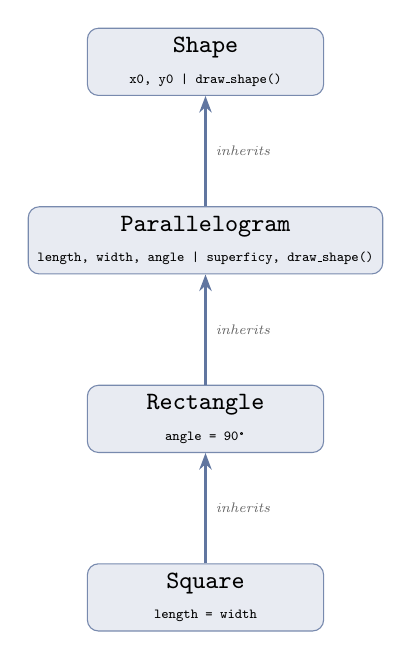
\begin{tikzpicture}[
    node distance = 1.4cm and 2.2cm,
    box/.style    = {draw, rounded corners=4pt, minimum width=3cm,
                     minimum height=0.8cm, align=center,
                     fill=headcolor!10, draw=headcolor!60, font=\ttfamily\small},
    arrow/.style  = {-{Stealth[length=6pt]}, thick, color=headcolor!70},
  ]
  \node[box] (shape) {\textbf{Shape}\\{\tiny x0, y0 | draw\_shape()}};
  \node[box, below=of shape] (para) {\textbf{Parallelogram}\\{\tiny length, width, angle | superficy, draw\_shape()}};
  \node[box, below=of para] (rect) {\textbf{Rectangle}\\{\tiny angle = 90°}};
  \node[box, below=of rect] (sq) {\textbf{Square}\\{\tiny length = width}};

  \draw[arrow] (para) -- (shape) node[midway, right, font=\tiny\itshape, color=pygray] {inherits};
  \draw[arrow] (rect) -- (para) node[midway, right, font=\tiny\itshape, color=pygray] {inherits};
  \draw[arrow] (sq)   -- (rect) node[midway, right, font=\tiny\itshape, color=pygray] {inherits};
\end{tikzpicture}
\end{center}

%% ─────────────────────────────────────────────
\subsection{Geometry of the Parallelogram}
%% ─────────────────────────────────────────────

The following figure shows a parallelogram with sides $\ell$ (base) and
$w$ (slant side) at angle $\theta$, with height $h$.

\begin{center}
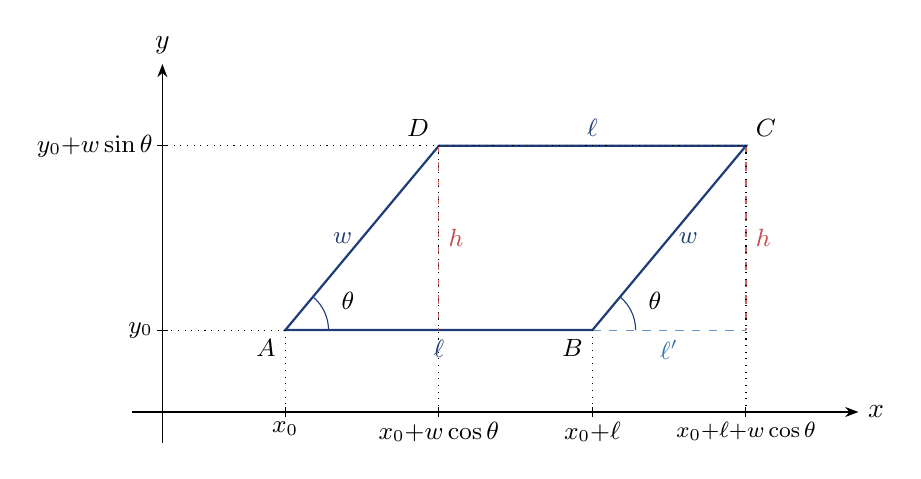
\begin{tikzpicture}[scale=1.3, >=Stealth]

  \coordinate (O)     at (0, 0);
  \coordinate (A)     at (1.2, 0.8);
  \coordinate (B)     at (4.2, 0.8);
  \coordinate (C)     at (5.7, 2.6);
  \coordinate (D)     at (2.7, 2.6);

  \coordinate (Ax)    at (1.2, 0);
  \coordinate (Bx)    at (4.2, 0);
  \coordinate (Cx)    at (5.7, 0);
  \coordinate (Dx)    at (2.7, 0);
  \coordinate (Ay)    at (0, 0.8);
  \coordinate (Cy)    at (0, 2.6);
  \coordinate (Bext)  at (5.5, 0.8);
  \coordinate (Dfoot) at (2.7, 0.8);
  \coordinate (Cfoot) at (5.7, 0.8);

  % Axes
  \draw[->] (-0.3, 0) -- (6.8, 0) node[right] {$x$};
  \draw[->] (0, -0.3) -- (0, 3.4) node[above] {$y$};

  % Parallelogram
  \draw[thick, color=headcolor] (A) -- (B) -- (C) -- (D) -- cycle;

  % Height dashes
  \draw[dashed, color=pyred!70] (D) -- (Dfoot);
  \draw[dashed, color=pyred!70] (C) -- (Cfoot);
  \draw[dashed, color=pyblue!60] (B) -- (Cfoot);

  % Projection dotted lines
  \draw[dotted] (A) -- (Ay);
  \draw[dotted] (A) -- (Ax);
  \draw[dotted] (B) -- (Bx);
  \draw[dotted] (C) -- (Cx);
  \draw[dotted] (D) -- (Dx);
  \draw[dotted] (C) -- (Cy);

  % Vertex labels
  \node[below left, font=\small]  at (A) {$A$};
  \node[below left, font=\small]  at (B) {$B$};
  \node[above right, font=\small] at (C) {$C$};
  \node[above left, font=\small]  at (D) {$D$};

  % Side labels
  \node[above, font=\small, color=headcolor] at ($(D)!0.5!(C)$) {$\ell$};
  \node[below, font=\small, color=headcolor] at ($(A)!0.5!(B)$) {$\ell$};
  \node[left,  font=\small, color=headcolor] at ($(A)!0.5!(D)$) {$w$};
  \node[right, font=\small, color=headcolor] at ($(B)!0.5!(C)$) {$w$};

  % Height labels
  \node[right, font=\small, color=pyred!80] at ($(D)!0.5!(Dfoot)$) {$h$};
  \node[right, font=\small, color=pyred!80] at ($(C)!0.5!(Cfoot)$) {$h$};
  \node[below, font=\small, color=pyblue!80] at ($(B)!0.5!(Cfoot)$) {$\ell'$};

  % Angle arcs
  \draw pic["$\theta$", draw=headcolor, angle radius=0.55cm, angle eccentricity=1.6, font=\small]
    {angle = B--A--D};
  \draw pic["$\theta$", draw=headcolor, angle radius=0.55cm, angle eccentricity=1.6, font=\small]
    {angle = Bext--B--C};

  % X-axis ticks
  \draw (1.2, 0.05) -- (1.2, -0.05);
  \draw (4.2, 0.05) -- (4.2, -0.05);
  \draw (5.7, 0.05) -- (5.7, -0.05);
  \draw (2.7, 0.05) -- (2.7, -0.05);
  \node[below, font=\small] at (Ax) {$x_0$};
  \node[below, font=\small] at (Bx) {$x_0{+}\ell$};
  \node[below, font=\footnotesize] at (Cx) {$x_0{+}\ell{+}w\cos\theta$};
  \node[below, font=\small] at (Dx) {$x_0{+}w\cos\theta$};

  % Y-axis ticks
  \draw (0.05, 0.8) -- (-0.05, 0.8);
  \node[left, font=\small] at (Ay) {$y_0$};
  \draw (0.05, 2.6) -- (-0.05, 2.6);
  \node[left, font=\small] at (Cy) {$y_0{+}w\sin\theta$};

\end{tikzpicture}
\end{center}

\vspace{0.5em}
\noindent\textbf{Trigonometric relations:}
\begin{align*}
  \cos\theta &= \frac{\ell'}{w} \quad\Longrightarrow\quad \ell' = w\cos\theta \\[4pt]
  \sin\theta &= \frac{h}{w}    \quad\Longrightarrow\quad h   = w\sin\theta
\end{align*}

\noindent\textbf{Vertex coordinates:}
\begin{align*}
  A &= (x_0,\ y_0) \\
  B &= (x_0 + \ell,\ y_0) \\
  C &= (x_0 + \ell + w\cos\theta,\ y_0 + w\sin\theta) \\
  D &= (x_0 + w\cos\theta,\ y_0 + w\sin\theta)
\end{align*}

The parallelogram is fully defined by $(x_0,\, y_0,\, \ell,\, w,\, \theta)$.

%% ─────────────────────────────────────────────
\subsection{The \texttt{Shape} and \texttt{Parallelogram} Classes}
%% ─────────────────────────────────────────────

We first define a base class \texttt{Shape} and then derive \texttt{Parallelogram} from it.

\begin{pycode}
import matplotlib.pyplot as plt  # Import the necessary library for plotting
from math import cos, sin, pi    # Import mathematical functions

class Shape:
    def __init__(self, x0: float, y0: float):
        self.x0 = x0  # Initialize the x-coordinate of the shape's reference point
        self.y0 = y0  # Initialize the y-coordinate of the shape's reference point

    def draw_shape(self):  # Define a method to draw the shape,
        pass               # which will be overridden in subclasses

# Define a class for parallelograms that inherits from the Shape class,
# since a parallelogram is a specific type of shape with additional
# properties and methods.
class Parallelogram(Shape):
    def __init__(self, x0: float, y0: float,
                 length: float, width: float, angle: float):
        super().__init__(x0, y0)  # Call the constructor of the parent class
        # Initialize the angle of the parallelogram in radians
        self.angle  = angle
        # Initialize the length of the parallelogram
        self.length = length
        # Initialize the width of the parallelogram
        self.width  = width
        # Calculate the height using the sine of the angle
        self.height = width * sin(angle)
        # Calculate the area using the formula: area = base * height
        self.superficy = length * self.height
        # Initialize the coordinates of point A (the reference point)
        self.point_A_x, self.point_A_y = x0, y0
        # Calculate the coordinates of point B by adding the length
        # to the x-coordinate of point A
        self.point_B_x, self.point_B_y = x0 + length, y0
        # Calculate the coordinates of point C by adding the length and
        # the horizontal component of the width to x0, and the vertical
        # component of the width to y0
        self.point_C_x = x0 + length + width * cos(angle)
        self.point_C_y = y0 + width * sin(angle)
        # Calculate the coordinates of point D by adding the horizontal
        # component of the width to x0, and the vertical component to y0
        self.point_D_x = x0 + width * cos(angle)
        self.point_D_y = y0 + width * sin(angle)

    # Define a method to print the description of the parallelogram,
    # including its properties: length, width, and the starting angle
    # (converted to degrees for better readability)
    def description(self):
        print(f"This is a {self.__class__.__name__.lower()} with the following properties:")
        print("Length: \t", self.length)
        print("Width: \t\t", self.width)
        # Convert angle from radians to degrees for a more intuitive understanding
        print("Angle (in degrees): \t", self.angle * 180 / pi)

    # Define the x-coordinates of the vertices of the parallelogram in order
    # (A, B, C, D, and back to A to close the shape)
    def draw_shape(self):
        data_x = [self.point_A_x, self.point_B_x,
                  self.point_C_x, self.point_D_x, self.point_A_x]
        data_y = [self.point_A_y, self.point_B_y,
                  self.point_C_y, self.point_D_y, self.point_A_y]
        labels = ['A', 'B', 'C', 'D']  # Define labels for the vertices
        for i, label in enumerate(labels):
            plt.text(data_x[i], data_y[i], label, fontsize=10,
                     ha='right', va='bottom')  # Annotate each vertex
        plt.plot(data_x, data_y, linestyle='-')  # Plot the parallelogram
        plt.axis('equal')    # Equal scaling for x and y axes
        plt.title(f"{self.__class__.__name__.lower()} representation")
        plt.show()   # Display the plot
        plt.close()  # Close the plot to free resources

    # Define a method to print the area (superficy) of the parallelogram,
    # which is calculated in the constructor
    def print_superficy(self):
        print(f"The superficy of the {self.__class__.__name__.lower()} is: {self.superficy}")
\end{pycode}

Instantiating and using \texttt{Parallelogram}:

\begin{pycode}
parallelogram1 = Parallelogram(2, 2, 6, 3, pi/4)
parallelogram1.description()
parallelogram1.print_superficy()
print(f'the superficy of the {parallelogram1.__class__.__name__.lower()} is: {parallelogram1.superficy}')
parallelogram1.draw_shape()
\end{pycode}

\begin{pyoutput}
This is a parallelogram with the following properties:\\
Length: 6 \\
Width:    3 \\
Angle (in degrees):45.0  \\
The superficy of the parallelogram is: 12.727922061357857 \\
the superficy of the parallelogram is: 12.727922061357857
\end{pyoutput}

\begin{center}
  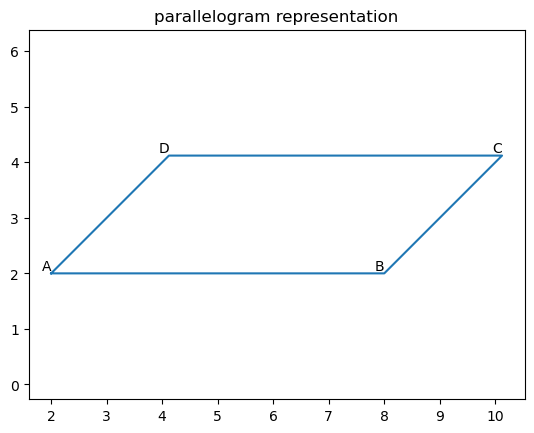
\includegraphics[width=0.7\linewidth]{output_1_1.png}
\end{center}

\begin{infobox}[How it works]
The \texttt{Shape} base class defines the interface (\texttt{draw\_shape})
without any implementation. \texttt{Parallelogram} inherits from
\texttt{Shape} and overrides \texttt{draw\_shape} with a concrete
Matplotlib-based drawing. This is both \emph{inheritance} (code reuse
through the class hierarchy) and \emph{polymorphism} (same method name,
different behaviour per class).
\end{infobox}

%% ─────────────────────────────────────────────
\subsection{The \texttt{Rectangle} and \texttt{Square} Classes}
%% ─────────────────────────────────────────────

A rectangle is a parallelogram with $\theta = 90^{\circ}$, and a square is a special rectangle with equal sides. Both inherit from the class above them in the
hierarchy.

\begin{pycode}
# Define a class for rectangles that inherits from the parallelogram class,
# since a rectangle is a special case of a parallelogram where the angle is
# always 90 degrees (pi/2 radians).
class Rectangle(Parallelogram):
    def __init__(self, x0: float, y0: float,
                 length: float, width: float):
        super().__init__(x0, y0, length, width, pi/2)

    # Define a method to print the description of the rectangle, including
    # its properties: length and width
    # (we can omit the angle since it's always 90 degrees for a rectangle)
    # We can also call the description method of the parent class to reuse
    # the code for printing length and width, but we override it here to
    # provide a more specific description for rectangles.
    def description(self):
        print(f"This is a {self.__class__.__name__.lower()} with the following properties:")
        print("Length: \t", self.length)
        print("Width: \t\t", self.width)

# Define a class for squares that inherits from the Rectangle class,
# since a square is a special case of a rectangle where length and width
# are equal.
class Square(Rectangle):
    def __init__(self, x0: float, y0: float, side: float):
        super().__init__(x0, y0, side, side)
        self.side = side  # Initialize the side length of the square,
                          # which is equal to both length and width

    # Define a method to print the description of the square, including
    # its properties: side length.
    # We override the parent's description to provide a more specific
    # description for squares.
    def description(self):
        print(f"This is a {self.__class__.__name__.lower()} with the following properties:")
        print("Side: \t", self.side)
\end{pycode}

Now we demonstrate all three classes together:

\begin{pycode}
# Create an instance of the parallelogram class and call its methods to
# demonstrate functionality
# (x0=2, y0=2, length=9, width=4, angle=pi/6 : 30 degrees)
parallelogram1 = Parallelogram(2, 2, 9, 4, pi/6)
parallelogram1.description()
print('the superficy of the parallelogram is:', parallelogram1.superficy)
parallelogram1.draw_shape()

# Create an instance of the Rectangle class and call its methods to
# demonstrate functionality
rectangle1 = Rectangle(1, 1, 10, 4)
rectangle1.description()
rectangle1.print_superficy()
print('the superficy of the rectangle is:', rectangle1.superficy)
rectangle1.draw_shape()

# Create an instance of the Square class and call its methods to
# demonstrate functionality
square1 = Square(3, 3, 3)
square1.description()
square1.print_superficy()
print('the superficy of the square is:', square1.superficy)
square1.draw_shape()
\end{pycode}

\begin{pyoutput}
This is a parallelogram with the following properties:\\
Length:          9\\
Width:           4\\
Angle (in degrees):      29.999999999999996\\
the superficy of the parallelogram is: 17.999999999999996
\end{pyoutput}

\begin{figure}[H]
  \centering
  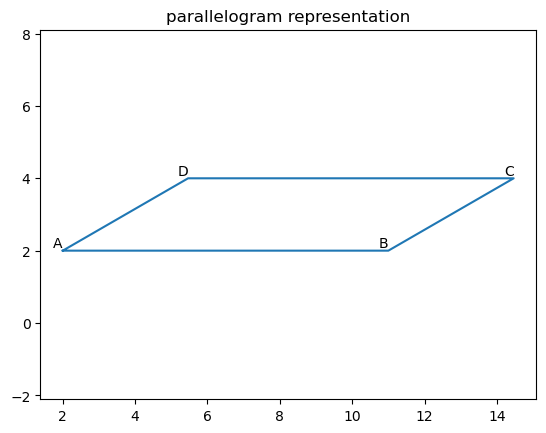
\includegraphics[width=0.65\linewidth]{output_3_1.png}
\end{figure}

\begin{pyoutput}
This is a rectangle with the following properties:\\
Length:          10\\
Width:           4\\
The superficy of the rectangle is: 40.0\\
the superficy of the rectangle is: 40.0
\end{pyoutput}

\begin{figure}[H]
  \centering
  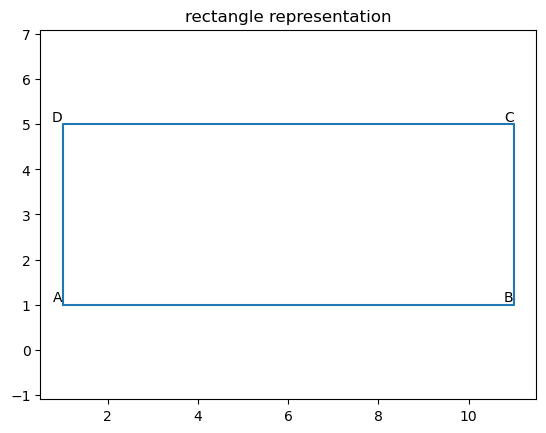
\includegraphics[width=0.65\linewidth]{output_3_3.png}
\end{figure}


\begin{pyoutput}
This is a square with the following properties:\\
Side:    3\\
The superficy of the square is: 9.0\\
the superficy of the square is: 9.0
\end{pyoutput}

\begin{figure}[H]
  \centering
  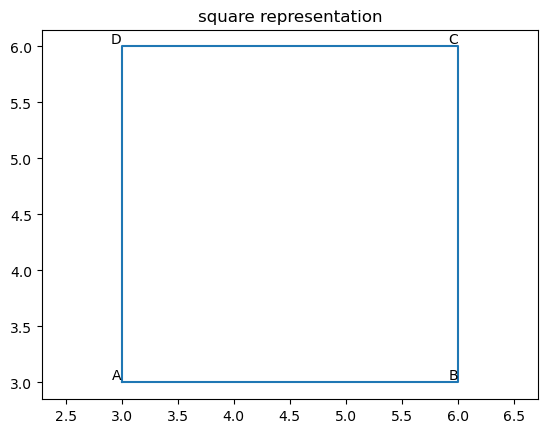
\includegraphics[width=0.65\linewidth]{output_3_5.png}
\end{figure}

%% ─────────────────────────────────────────────
\section{Summary}
%% ─────────────────────────────────────────────

\begin{enumerate}[leftmargin=1.5em, itemsep=4pt]
  \item We import \texttt{matplotlib.pyplot} for plotting and \texttt{math} for trigonometric functions.
  \item \texttt{Shape} defines the base interface with an \texttt{\_\_init\_\_} method for coordinates and a placeholder \texttt{draw\_shape} method.
  \item \texttt{Parallelogram} inherits from \texttt{Shape} and extends it with length, width, angle, height, and area. It overrides \texttt{draw\_shape} to render the shape with Matplotlib.
  \item \texttt{Rectangle} inherits from \texttt{Parallelogram}, fixing the angle at $90^{\circ}$ and overriding \texttt{description}.
  \item \texttt{Square} inherits from \texttt{Rectangle}, constraining length\,$=$\,width and overriding \texttt{description}.
  \item \textbf{Polymorphism} is demonstrated through \texttt{description()} — the same call produces different output for each class — and through \texttt{print\_superficy()} and
        \texttt{draw\_shape()}, which are inherited and shared across the entire hierarchy.
\end{enumerate}

\begin{mytip}[Key Takeaway]
The \texttt{super()} call is the mechanism that chains constructors up
the hierarchy. Each subclass calls its parent's \texttt{\_\_init\_\_}
to reuse shared initialisation logic, adding only the parameters it
needs — a clean expression of the DRY principle.
\end{mytip}

\vspace{2em}
\noindent\rule{\linewidth}{0.4pt}
\vspace{0.4em}

\noindent{\small\color{pygray}
  Source code available at:
  \href{https://github.com/Abdou-fi/Python-OOP}{\texttt{github.com/Abdou-fi/Python-OOP}}
  \hfill \textit{Encapsulation and inner classes will be covered in a future article.}
}

\end{document}